%\documentclass[conference,final]{IEEEtran}
%\documentclass{acm_proc_article-sp}

\documentclass{sig-alternate}

%\documentclass{acm_proc_article-sp}

\usepackage[numbers, sort, compress]{natbib}
\usepackage{graphicx}
\usepackage{amsmath}
\usepackage{amssymb}
\usepackage{color}
\usepackage{ifpdf}

\usepackage{dcolumn}
\usepackage{float}
\usepackage[utf8]{inputenc}
\usepackage{multirow}
\usepackage{rotating}

\usepackage[tight]{subfigure}



%\usepackage[numbers, sort, compress]{natbib}
%\usepackage{latex8}
%\usepackage{float}
%\usepackage{times}    
\usepackage{url}
\usepackage{listings}   
\usepackage{paralist}    
\usepackage{wrapfig}    
%\usepackage[small,it]{caption}
\usepackage{multirow}
\usepackage{ifpdf}
%\usepackage{srcltx}
%\usepackage{subfigure}
\usepackage{xspace}
\usepackage{keyval}  
\usepackage{color}

\definecolor{listinggray}{gray}{0.95}
\definecolor{darkgray}{gray}{0.7}
\definecolor{commentgreen}{rgb}{0, 0.4, 0}
\definecolor{darkblue}{rgb}{0, 0, 0.4}
\definecolor{middleblue}{rgb}{0, 0, 0.7}
\definecolor{darkred}{rgb}{0.4, 0, 0}
\definecolor{brown}{rgb}{0.5, 0.5, 0}

\usepackage[normalem]{ulem}
\makeatletter
\def\cyanuwave{\bgroup \markoverwith{\lower3.5\p@\hbox{\sixly \textcolor{cyan}{\char58}}}\ULon}
\def\reduwave{\bgroup \markoverwith{\lower3.5\p@\hbox{\sixly \textcolor{red}{\char58}}}\ULon}
\def\blueuwave{\bgroup \markoverwith{\lower3.5\p@\hbox{\sixly \textcolor{blue}{\char58}}}\ULon}
\font\sixly=lasy6 % does not re-load if already loaded, so no memory problem.
\makeatother


\begin{document}
%\conferenceinfo{WOODSTOCK}{'97 El Paso, Texas USA}
% \conferenceinfo{ECMLS'11,} {June 8, 2011, San Jose, California, USA.}
% \CopyrightYear{2011}
% \crdata{978-1-4503-0702-4/11/06}
% \clubpenalty=10000
% \widowpenalty = 10000

%!TEX root = sc12/pstar-sc2012-ieee.tex
\newif\ifdraft
%\drafttrue
\ifdraft
\newcommand{\onote}[1]{ {\textcolor{cyan} { (***Ole: #1) }}}
\newcommand{\terminology}[1]{ {\textcolor{red} {(Terminology used: \textbf{#1}) }}}
\newcommand{\owave}[1]{ {\cyanuwave{#1}}}
\newcommand{\jwave}[1]{ {\reduwave{#1}}}
\newcommand{\alwave}[1]{ {\blueuwave{#1}}}
\newcommand{\jhanote}[1]{ {\textcolor{red} { ***shantenu: #1 }}}
\newcommand{\alnote}[1]{ {\textcolor{blue} { ***andreL: #1 }}}
\newcommand{\amnote}[1]{ {\textcolor{blue} { ***andreM: #1 }}}
\newcommand{\smnote}[1]{ {\textcolor{brown} { ***sharath: #1 }}}
\newcommand{\msnote}[1]{ {\textcolor{cyan} { ***mark: #1 }}}
\newcommand{\note}[1]{ {\textcolor{magenta} { ***Note: #1 }}}
\else
\newcommand{\onote}[1]{}
\newcommand{\terminology}[1]{}
\newcommand{\owave}[1]{#1}
\newcommand{\jwave}[1]{#1}
\newcommand{\alnote}[1]{}
\newcommand{\amnote}[1]{}
\newcommand{\athotanote}[1]{}
\newcommand{\smnote}[1]{}
\newcommand{\jhanote}[1]{}
\newcommand{\msnote}[1]{}
\newcommand{\note}[1]{}
\fi

\newcommand{\pilot}{Pilot\xspace}
\newcommand{\pilots}{Pilots\xspace}
\newcommand{\pilotjob}{Pilot-Job\xspace}
\newcommand{\pilotjobs}{Pilot-Jobs\xspace}
\newcommand{\computeunit}{Compute Unit\xspace}
\newcommand{\computeunits}{Compute Units\xspace}
\newcommand{\cu}{CU\xspace}
\newcommand{\cus}{CUs\xspace}
\newcommand{\cs}{Compute Service\xspace}
\newcommand{\css}{Compute Services\xspace}
\newcommand{\pcs}{Pilot Compute Service\xspace}
\newcommand{\dataunit}{Data Unit\xspace}
\newcommand{\dataunits}{Data Unit\xspace}
\newcommand{\du}{DU\xspace}
\newcommand{\dus}{DUs\xspace}
\newcommand{\pilotdata}{Pilot-Data\xspace}
\newcommand{\pd}{PD\xspace}
\newcommand{\pds}{Pilot Data Service\xspace}
\newcommand{\pdss}{Pilot Data Services\xspace}
\newcommand{\su}{SU\xspace}
\newcommand{\sus}{SUs\xspace}
\newcommand{\schedulableunit}{Schedulable Unit\xspace}
\newcommand{\schedulableunits}{Schedulable Units\xspace}
\newcommand{\cc}{c\&c\xspace}
\newcommand{\CC}{C\&C\xspace}

\lstdefinestyle{myListing}{
  frame=single,   
  backgroundcolor=\color{listinggray},  
  %float=t,
  language=C,       
  basicstyle=\ttfamily \footnotesize,
  breakautoindent=true,
  breaklines=true
  tabsize=2,
  captionpos=b,  
  aboveskip=0em,
  belowskip=-2em,
  %numbers=left, 
  %numberstyle=\tiny
}      

\lstdefinestyle{myPythonListing}{
  frame=single,   
  backgroundcolor=\color{listinggray},  
  %float=t,
  language=Python,       
  basicstyle=\ttfamily \footnotesize,
  breakautoindent=true,
  breaklines=true
  tabsize=2,
  captionpos=b,  
  %numbers=left, 
  %numberstyle=\tiny
}

\newcommand{\up}{\vspace*{-1em}}
\newcommand{\upp}{\vspace*{-0.5em}}
\newcommand{\numrep}{8 }
\newcommand{\samplenum}{4 }
\newcommand{\tmax}{$T_{max}$ }
\newcommand{\tc}{$T_{C}$ }
\newcommand{\tcnsp}{$T_{C}$}
\newcommand{\bj}{BigJob}

%  \setlength{\parskip}{0.05ex} % 1ex plus 0.5ex minus 0.2ex}
%  \setlength{\parsep}{0pt}
%  %\setlength{\headsep}{0pt}
%  \setlength{\topskip}{0pt}
%  \setlength{\topmargin}{0pt}
%  %\setlength{\topsep}{0pt}
%  \setlength{\partopsep}{0pt}

% This is now the recommended way for checking for PDFLaTeX:


\ifpdf
\DeclareGraphicsExtensions{.pdf, .jpg, .tif}
\else
\DeclareGraphicsExtensions{.eps, .jpg}
\fi

\tolerance=1000
\hyphenpenalty=10


% \author{
%   Andre Luckow$^{1}$, Mark Santcroos$^{2,1}$, Ole Weidner$^{1}$, Andre Merzky$^{1}$, Sharath Maddineni$^{1}$, Shantenu Jha$^{3,1*}$\\[0.5em]
%   \small{\emph{$^{1}$Center for Computation \& Technology, Louisiana State University, USA}}\\[-0.3em]
%   \small{\emph{$^{2}$Bioinformatics Laboratory, Academic Medical Center, University of Amsterdam, The Netherlands}}\\[-0.3em]
%   \small{\emph{$^{3}$ Rutgers University, Piscataway, NJ 08854, USA}}\\[-0.3em]
% %  \small{\emph{$^{4}$ School of Informatics, University of Edinburgh, UK }}\\[-0.3em]
%   \small{\emph{$^{*}$Contact Author: \texttt{shantenu.jha@rutgers.edu}}}\\[-0.3em]
%   \up\up\up }


\title{P*: A Model of Pilot-Abstractions\up}
\numberofauthors{5}
\author{
\alignauthor Andre Luckow\\
       \affaddr{Center for Computation\newline and Technology}\\
       \affaddr{Louisiana State University}\\
       \affaddr{216 Johnston}\\
       \affaddr{Baton Rouge, LA} \\
       \email{aluckow@cct.lsu.edu}
\and
\alignauthor Mark Santcroos\\
       \affaddr{Bioinformatics Laboratory}\\
       \affaddr{Academic Medical Center}\\
       \affaddr{University of Amsterdam}\\
       \affaddr{Meibergdreef 9}\\
       \affaddr{Amsterdam, The Netherlands}
       \email{m.a.santcroos@amc.uva.nl}
\and
\alignauthor Ole Weidner\\
       \affaddr{Center for Computation\newline and Technology}\\
       \affaddr{Louisiana State University}\\
       \affaddr{216 Johnston}\\
       \affaddr{Baton Rouge, LA}
       \email{oweidner@cct.lsu.edu}
\and
\alignauthor Andre Merzky\\
       \affaddr{Center for Computation\newline and Technology}\\
       \affaddr{Louisiana State University}\\
       \affaddr{216 Johnston}\\
       \affaddr{Baton Rouge, LA}
       \email{amerzky@cct.lsu.edu}
\alignauthor Sharath Maddineni\\
       \affaddr{Center for Computation\newline and Technology}\\
       \affaddr{Louisiana State University}\\
       \affaddr{216 Johnston}\\
       \affaddr{Baton Rouge, LA}
       \email{smaddineni@cct.lsu.edu}
\and
\alignauthor Shantenu Jha\\
      \affaddr{CAC/ECE}\\
     \affaddr{Rutgers University}\\
      \affaddr{94 Brett Road}\\
      \affaddr{Piscataway, NJ}
     \email{shantenu.jha@rutgers.edu}
}

\date{}

\maketitle

\begin{abstract} 
  In spite of broad uptake, there does not exist a well defined,
  unifying conceptual model of \pilotjobs which can be used to define,
  compare and contrast different implementations. This presents a
  barrier to extensibility and interoperability. This paper is an
  attempt to (i) provide a minimal but complete model (P*) of
  \pilotjobs, (ii) establish the generality of the P* Model by mapping
  various existing and well known \pilotjob frameworks such as Condor
  and DIANE to P*, (iii) derive an interoperable and extensible API
  for the P* Model (Pilot-API), (iv) validate the implementation of
  the Pilot-API by concurrently using multiple {\it distinct}
  pilot-job frameworks on distinct production distributed
  cyberinfrastructures, and (v) apply the P* Model to \pilotdata.
\end{abstract}
%\category{H.4}{Information Systems Applications}{Miscellaneous}
%terms{Theory}
%\keywords{ACM proceedings, \LaTeX, text tagging}
%\up\up

\section{Introduction and Overview} 

Distributed cyber/e-infrastructure is by definition comprised of a set
of resources that is fluctuating -- growing, shrinking, changing in
load and capability (in contrast to a static resource utilization
model of traditional parallel and cluster computing systems).  The
ability to utilize a dynamic resource pool is thus an important
attribute of any application that needs to utilize distributed
cyberinfrastructure (DCI) efficiently. \pilotjobs (PJ) provide an
effective abstraction for dynamic execution and resource utilization
in a distributed context. As a consequence of providing a simple
approach for decoupling workload management and resource
assignment/scheduling, \pilotjobs have been one of the most successful
abstractions in distributed computing.  Not surprisingly, there are
multiple, distinct and incompatible implementations of
pilot-jobs. Often these implementations are strongly coupled to the
distributed cyberinfrastructure they were originally designed for.

% The fundamental reason for the success of the PJ abstraction is that
% PJ liberate applications/users from the challenging requirement of
% mapping specific tasks onto explicit heterogeneous and dynamic
% resource pools.  PJ also thus shields application from having to
% load-balance tasks across such resources.  The \pilotjob abstraction
% is also a promising route to address specific requirements of
% distributed scientific applications, such as coupled-execution and
% application-level scheduling~\cite{ko-efficient,DBLP:conf/hpdc/KimHMAJ10}.

% A variety of PJ frameworks have emerged:
% Condor-G/ Glide-in~\cite{condor-g}, Swift~\cite{Wilde2011},
% DIANE~\cite{Moscicki:908910}, DIRAC~\cite{1742-6596-219-6-062049},
% PanDA~\cite{1742-6596-219-6-062041}, ToPoS~\cite{topos},
% Nimrod/G~\cite{10.1109/HPC.2000.846563}, Falkon~\cite{1362680} and
% MyCluster~\cite{1652061} to name a few. Although they are all, for the
% most parts, functionally equivalent -- they support the decoupling of
% workload submission from resource assignment -- it is often impossible
% to use them interoperably or even just to compare them functionally or
% qualitatively.  The situation is reminiscent of the proliferation of
% functionally similar yet incompatible workflow systems, where in spite
% of significant a posteriori effort on workflow system extensibility
% and interoperability (thus providing post-facto justification of its
% needs), these objectives remains difficult if not infeasible.

Our objective is to provide a minimal, but complete model of
\pilotjobs: The P* Model provides a conceptual basis to compare and
contrast different PJ frameworks.  We discuss how existing and widely
used \pilotjob frameworks, can be used through the Pilot-API. We
perform experiments and performance measurements used to characterize
the workings of the Pilot-API and to demonstrate interoperability
across middleware, platform and different PJ frameworks.  A natural
and logical extension of the P* Model arises from the need to extend
it to include data in addition to computational tasks.  This leads to
analogous abstraction to the \pilotjob: the \emph{\pilotdata (PD)}
abstraction.  The potentially consistent treatment of data and compute
suggests symmetrical compute and data elements in the model; thus we
refer to this model as the P* Model ("P-star").


% It is worth noting that \pilotjobs are used on every major
% national and international DCI, including NSF/XSEDE,
% NSF/DOE Open Science Grid, EU EGI and others, to support hundreds and
% thousands of tasks daily, thus we believe the impact and validation of
% this paper lies in its ability to not only influence but also bridge
% the theory and practice of \pilotjobs, and thus multiple domains of
% science dependent on distributed cyberinfrastructure.





%  which is also partly motivated by
% the status of the usage and availability of the pilot abstraction
% vis-\`{a}-vis the current landscape of distributed applications and
% cyberinfrastructure.

 % Collectively pilot-jobs support
% hundreds of thousands if not millions of tasks every day.  As we will
% show, the Pilot-API provides a single uniform API to PJ-frameworks
% thus providing for the first time... removing barriers to...
% \jhanote{fix..}


\section{The P* Model of Pilot-\\Abstractions}
\label{sec:pilot-model}

The P* model is derived from an analysis of many \pilotjob
implementations; based upon this analysis, we first present the common
{\it elements} of the P* Model, followed by a description of the {\it
  characteristics} that determine the interaction of these elements
and the overall functioning of a \pilotjob framework that is
consistent with the P* Model.

\begin{figure}[t]
    \centering
    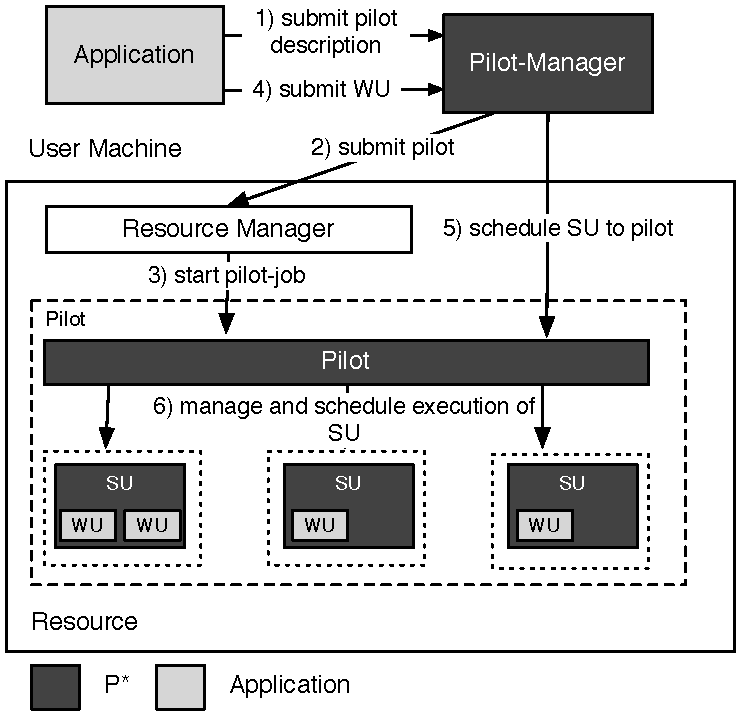
\includegraphics[width=0.48\textwidth]{figures/pstar_model_single.pdf}
    \caption{ \textbf{P* Model: Elements, Characteristics and
        Interactions:} The manager has two functions: it manages 1)
      Pilots (step 1-3) and 2) the execution of \cus. After a \cu is
      submitted to the manager, it transitions to an \su, which is
      scheduled to a \pilot by the PM. The \pilot then schedules the
      \su to an available resource.  }
    \label{fig:figures_pstar}
\end{figure}

\noindent 
\subsection{Elements of the P* Model}


\noindent This sub-section defines the elements of the P* Model:


%\alnote{use pilot NOT pilot-job}
\noindent$\bullet$ \textbf{\pilot (Pilot-Compute):} The \pilot is the
  entity that actually gets submitted and scheduled on a resource.
% via the resource's RM system. 
  The PJ provides application (user)
  level control and management of the set of allocated resources.

  % and is responsible for the execution of \alwave{SUs/tasks}
  % onto the resource.

  % \alnote{\textbf{The RM assigns a slice of the Resource to the
  %     pilot -- that pilot then acts as RM for that resource slice.}
  %   I think simply equating a pilot with a RM is bit too
  %   simplistic. In a sense it is a application-level resource
  %   manger. Not sure what to do}

\noindent$\bullet$ \textbf{\computeunit  (\cu):} A \cu  encapsulates a 
  self-contained piece of work (a task) specified by the application that is
  submitted to the \pilotjob framework. There is no intrinsic notion
  of resource associated with a \cu.

\noindent$\bullet$ \textbf{Scheduling Unit (SU):} SUs are the units of 
  scheduling, internal to the P* Model, i.e., it is not known by or
  visible to an application. Once a \cu is
  under the control of the \pilotjob framework, it is assigned
  to an SU.
  % An SU is created after the submission of
  %   a \cu, i.\,e.\ once a \cu \ has been passed into the control of the
  %   pilot-job framework. 
%  \jhanote{Could we say: Once a \cu has been
%    passed into the control of the pilot-job framework, it is assigned
%    to an SU} \alnote{sounds good. done.}

\noindent$\bullet$ \textbf{Pilot-Manager (PM):} The PM is responsible for (i)
  orchestrating the interaction between the \pilots as well as the
  different components of the P* Model (\cus, \sus) and (ii) decisions
  related to internal resource assignment (once resources have been
  acquired by the \pilotjob).  For example, an SU can consists of one
  or more \cus. Further, \cus and \sus can be combined and aggregated;
  the PM determines how to group them, when \sus are scheduled and
  executed on a resource via the \pilot, as well as how many resources
  to assign to an SU.

An application kernel is the actual binary that gets executed.  The
application utilizes a PJ framework to execute multiple instances of
an application kernel (an ensemble) or alternatively instances of
multiple different application kernels (a workflow).  To execute an
application kernel, an application must define a \cu \ specifying the
application kernel as well as other parameters. This \cu \ is then
submitted to the PM (as an entry point to the
\pilotjob framework), where it transitions to an SU. The PM is then
responsible for scheduling the SU onto a \pilot and then onto a
physical resource.  As shown in table~\ref{table:bigjob-saga-diane}, 
the above elements can be mapped to specific entities in many \pilotjobs 
in existence and use; often more than one logical element may be rolled 
into a specific entity in a \pilotjob.

% \textbf{Diane Definition of Terms: } The computation consists of
% many worker processes which communicate with one master process (the
% worker processes do not need to share the filesystem nor
% memory). The ensemble of computation is called a run and it consists
% of many tasks which may be executed in parallel. A task is defined
% as a set of parameters which are produced by the RunMaster (running
% on a master node) and consumed by the WorkerAgent (running on a
% worker node).
% 
% from 
% 
% DIANE assumes the master-worker computing model (Fig.
% 1). Client sends job parameters to the Planner which partitions
% the job into smaller tasks executed by the Workers. Integrator
% is responsible for merging the results of task execution and
% sending the final job outcome to the Client.


\subsection{Characteristics of P* Model}
\label{sec:p_star_elements}
\alnote{the characteristics can be removed in my opinion}

%\jhanote{Why not have Binding as the first characteristics?}

% To understand % the degrees of freedom that any specific pilot-job
% % implementation must constraint as well as
% the functioning of
% pilot-jobs implementation, 
%These characteristics are integral components of the P* Model, in
% Further, these properties are important for the implementation of
% P*.  list several characteristics.
% The way the coordination between the different elements
% is handled is required to understand a PJ implementation.
 
We propose a set of fundamental properties/characteristics that
describe the interactions between the elements, and thus aid in the
description of P* Model.

% \alnote{ok} \jhanote{One strategy could be to not define the different
%   types, but just list/enumerate? Akin to Communication. i.e. explain
%   what coordination is for, what is being coordinated, how (the 3
%   types)}

\textbf{Coordination:} The coordination characteristics describe how
various elements of the P* Model, i.\,e.\ the PM, the \pilot, the \cus
and the SUs, interact. A common coordination pattern is master/worker
(M/W). %  the PM represents the master process that controls a set of
% worker processes, the \pilots. The point of decision making is the
% master process. In addition to the \emph{centralized} M/W, M/W can
% also be deployed \emph{hierarchically}.  Alternatively, coordination
% between the elements, in particular the \pilots, can be performed so as
% to be \emph{decentralized}, i.\,e.\ without central decision making
% point.

%\input{sectionIII-comments}

\textbf{Communication:} The communication characteristics describes
the mechanisms for data exchange between the elements of the P* Model:
e.\,g.\ messages (point-to-point, all-to-all, one-to-all, all-to-one,
or group-to-group).
		
\textbf{Scheduling:} The scheduling characteristics describes the
process of mapping a SU to resources via a \pilot and potential
multiple levels of scheduling. Scheduling has a spatial component
(which SU is executed on which \pilot?) but also a temporal component
(when to bind?). % The different scheduling decisions that need to be
% made are representative of multi-level scheduling decisions that are
% often required in distributed environments.  For example, when should
% a SU be bound to a \pilot?  An SU can be bound to a \pilot either before
% the \pilot has in turn been scheduled ({\it early} binding), whereas
% {\it late} binding occurs if the SU is bound after the \pilot has been
% scheduled.  In general, there are multiple-levels at which scheduling
% decisions, i.e., resource selection and binding, are made.

% The term {\it agent}, although not a part of the P* Model, finds
% mention when discussing implementations. For the purposes of this
% paper, an agent refers to a ``proxy process'' that has some decision
% making capability, and could aid the implementation of one or more of
% the characteristics of the P* Model -- coordination, communication,
% scheduling, within a \pilotjob framework.  These agents can be used to
% enforce a set of (user-defined) policies (e.g.  resource capabilities,
% data/compute affinities, etc.) and heuristics.

% \subsection{Putting it all together} 

% Figure~\ref{fig:figures_pstar} illustrates the interactions between
% the elements of the P* Model. First, the application specifies the
% capabilities of the resources required using a \pilotjob description
% (step 1). The PM then submits the necessary number of \pilots to
% fulfill the resource requirements of the application (step~2). Each
% \pilot is queued at the resource manager, which is responsible for
% starting the \pilot (step~3). There can be variations of this flow:
% while in the described model, the application defines the required
% resources, the PM could also decide based on the submitted \cu \
% workload whether and when it submits new \pilots.

% %\jhanote{What about the Resource Manager? Is it part of the resource}

% The application can submit \cus to the PM at any time (step~4). A
% submitted \cu \ becomes an SU, i.\,e.\ the PM is now in control of
% it. In the simplest case one \cu \ corresponds to one SU; however,
% SUs can be combined and aggregated to optimize throughputs and
% response times. Commonly, a hierarchical M/W model for coordination
% is used internally: the PM uses M/W to coordinate a set of \pilots,
% the \pilot itself functions as manager for the execution of the
% assigned SUs.


% Scheduling decisions can be made on multiple levels. The PM is responsible for
% selecting a \pilot for an SU (step 5). A \pilot is bound to a physical resource
% on which it is responsible for a particular resource set. Once a SU has been
% scheduled to a \pilot, the \pilot decides when and on which part of the resource
% an SU is executed.

% Further, the \pilot manages the subsequent execution of an SU
% (step~6).  There can be variations of this flow.  PJ frameworks with
% decentralized decision making e.\,g.\ often utilize autonomic agents
% that accept respectively pull SUs according to a set of defined
% policies.


\begin{table*}[t]
 
 \centering
 \begin{tabular}{|p{3.1cm}|p{2.5cm}|p{2.0cm}|p{3.3cm}|p{3.5cm}|}
  \hline
  \textbf{P* Element}    &\textbf{BigJob} &\textbf{DIANE} &\textbf{Condor-G/Glide-in}     &\textbf{Swift/Coaster}  \\\hline
  Pilot-Manager          &BigJob Manager  & RunMaster     & condor\_master,\newline 
                                                            condor\_collector,\newline 
                                                            condor\_negotiator,\newline 
                                                            condor\_schedd                &Coaster Service         \\\hline
  \pilot                 &BigJob Agent    & Worker Agent  &condor\_master,\newline
                                                           condor\_startd                 &Coaster Worker          \\\hline
  \computeunit  \ (CU)   &Task            &Task           &Job                            &Application Interface\newline Function (Swift Script)\\\hline
  Scheduling Unit \ (SU) &Sub-Job         &Task           &Job                            &Job                     \\\hline
% Dynamic Resources &no/yes &yes (AgentFactories)\\
% \hline
 \end{tabular}
 \caption{\textbf{Mapping P* elements and PJ Frameworks:} While each
   PJ framework maintains its own vocabulary, each of the P* elements
   can be mapped to one (or more) components of the different PJ
   frameworks. \jhanote{this table should definitely stay in my opinion}
 } 
 \label{table:bigjob-saga-diane}
\end{table*}


% \section{Pilot-API: A Uniform API to Heterogeneous PJ Frameworks}
% \label{sec:pilot-api}

\subsection{Experiments and Results}
 \label{sec:exp_res}

\jhanote{we need 1 plot here... which one is the Q}
\alnote{I propose to put figure 7 here. It shows that we can use 
	different PJ frameworks, but does not give to many things away, 
	such as the concurrent usage of different PJ frameworks and 
	infrastructures.}
 
\begin{figure}[t]
 \centering
 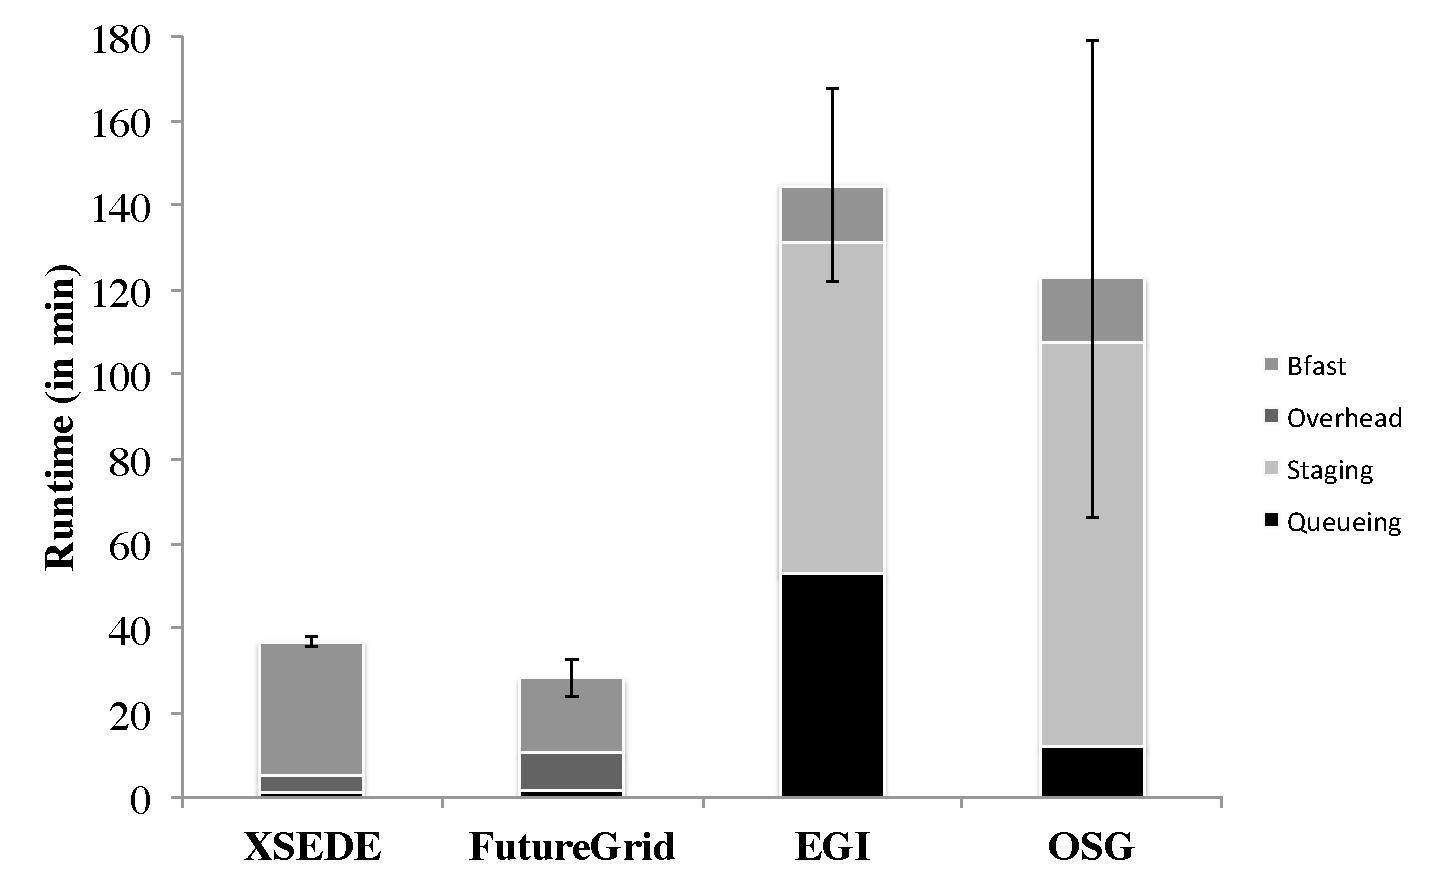
\includegraphics[width=0.48\textwidth]{perf/interop/128-bfast-egi-fg-xsede-osg.pdf}
 \caption{\textbf{PJ Framework Performance on XSEDE, FutureGrid, EGI and 
  OSG:} Running 128 BFAST match tasks on 128 cores. Each experiment is
  repeated at least 3 times. The longer runtimes on EGI and OSG are
  mainly caused by the longer queuing times. Additionally, 
	both infrastructure require the staging of all input files. }
	\label{fig:perf_perf-bfast-bj}
\end{figure}


\section{P* as a Model for Pilot-Data}
\label{sec:pilot-data}

While Pilot-Jobs efficiently support late-binding of \computeunits and
resources, the management of data in distributed systems remains a
challenge due to various reasons: (i) the placement of data is often
decoupled from the placement of Compute Units and Pilots, i.\,e.\ the
application must often manually stage in and out its data using simple
scripts; (ii) heterogeneity, e.\,g.\ with respect to storage,
filesystem types and paths, often prohibits or at least complicates
late binding decisions; (iii) higher-level abstraction that allow
applications to specify their data dependencies on an abstract,
logical level (rather than on file basis) are not available; (iv) due
to lack of a common treatment for compute and data, optimizations of
data/compute placements are often not possible.  In addition,
applications must cope with various other challenging, data-related
issues, e.\,g.\ varying data sources (such as sensors and/or other
application components), fluctuating data rates, transfer failures,
optimizations for different queries, data-/compute co-location
etc. While these issues can be in principal handled in an
application-specific way, the usage of higher-level abstractions, such
as a common \pilot-based abstraction for compute and data is
preferable.  This motivates an analogous abstraction that we call
\emph{\pilotdata (PD)}. PD provides late-binding capabilities for data
by separating the allocation of physical storage and application-level
data units. Further, it provides an abstraction for expressing and
managing relationships between data units and/or compute units. These
relationships are referred to as \emph{affinities}.

\section{Discussion and Future Work}
 \label{sec:discussion-future-work}

 \jhanote{best to rewrite..}

% The primary intellectual contribution of this work has been the
% development of the P* Model, the mapping of P* elements to PJ
% frameworks such as DIANE and Condor-G/Glide-in and the design and
% development of the Pilot-API -- that reflects the P* elements and
% characteristics.
 
% The P* Model provides a common abstract model for describing and
% characterizing Pilot-abstractions.  We validate the P* Model by
% demonstrating that the most widely used PJ frameworks, viz., DIANE and
% Condor-G/Glide-in can be compared, contrasted and analyzed using this
% analytical framework.  Furthermore we demonstrate the use of the
% Pilot-API -- which provides a common access layer to different PJ
% frameworks, with multiple PJ frameworks over distributed production
% cyberinfrastructure, such as XSEDE, OSG, EGI and FutureGrid. The
% Pilot-API also enables the concurrent use of multiple PJ frameworks,
% thus providing interoperability and extensibility.  Although the aim
% of our experiments is the demonstration of the interoperable use of
% hitherto distinct and disjoint \pilotjobs, in the process we highlight
% the performance advantages that can emanate from the ability to
% seamlessly distribute (I/O intensive) workloads in a scalable manner.


% \section*{Acknowledgements}
% This work is funded by NSF CHE-1125332 (Cyber-enabled Discovery and
% Innovation), HPCOPS NSF-OCI 0710874 award, NSF-ExTENCI (OCI-1007115)
% and NIH Grant Number P20RR016456 from the NIH National Center For
% Research Resources. Important funding for SAGA has been provided by
% the UK EPSRC grant number GR/D0766171/1 (via OMII-UK) and the
% Cybertools project (PI Jha) NSF/LEQSF
% (2007-10)-CyberRII-01. SJ acknowledges the e-Science Institute,
% Edinburgh for supporting the research theme. ``Distributed Programming
% Abstractions'' \& 3DPAS. MS is sponsored by the program of BiG Grid,
% the Dutch e-Science Grid, which is financially supported by the
% Netherlands Organisation for Scientific Research, NWO. SJ acknowledges
% useful related discussions with Jon Weissman (Minnesota) and Dan Katz
% (Chicago). We thank J Kim (CCT) for assistance with BFAST.  This work
% has also been made possible thanks to computer resources provided by
% TeraGrid TRAC award TG-MCB090174 (Jha) and BiG Grid.  This document
% was developed with support from the US NSF under Grant No. 0910812 to
% Indiana University for ``FutureGrid: An Experimental, High-Performance
% Grid Test-bed''.

% %\bibliographystyle{plain}
% %\bibliographystyle{IEEEtranS}
% \bibliographystyle{IEEEtran}
% %\bibliography{pilotjob,saga,saga-related}
% \bibliography{pstar-hpdc2012}

\end{document}
